\documentclass[twoside]{book}

% Packages required by doxygen
\usepackage{fixltx2e}
\usepackage{calc}
\usepackage{doxygen}
\usepackage{graphicx}
\usepackage[utf8]{inputenc}
\usepackage{makeidx}
\usepackage{multicol}
\usepackage{multirow}
\PassOptionsToPackage{warn}{textcomp}
\usepackage{textcomp}
\usepackage[nointegrals]{wasysym}
\usepackage[table]{xcolor}

% Font selection
\usepackage[T1]{fontenc}
\usepackage{mathptmx}
\usepackage[scaled=.90]{helvet}
\usepackage{courier}
\usepackage{amssymb}
\usepackage{sectsty}
\renewcommand{\familydefault}{\sfdefault}
\allsectionsfont{%
  \fontseries{bc}\selectfont%
  \color{darkgray}%
}
\renewcommand{\DoxyLabelFont}{%
  \fontseries{bc}\selectfont%
  \color{darkgray}%
}
\newcommand{\+}{\discretionary{\mbox{\scriptsize$\hookleftarrow$}}{}{}}

% Page & text layout
\usepackage{geometry}
\geometry{%
  a4paper,%
  top=2.5cm,%
  bottom=2.5cm,%
  left=2.5cm,%
  right=2.5cm%
}
\tolerance=750
\hfuzz=15pt
\hbadness=750
\setlength{\emergencystretch}{15pt}
\setlength{\parindent}{0cm}
\setlength{\parskip}{0.2cm}
\makeatletter
\renewcommand{\paragraph}{%
  \@startsection{paragraph}{4}{0ex}{-1.0ex}{1.0ex}{%
    \normalfont\normalsize\bfseries\SS@parafont%
  }%
}
\renewcommand{\subparagraph}{%
  \@startsection{subparagraph}{5}{0ex}{-1.0ex}{1.0ex}{%
    \normalfont\normalsize\bfseries\SS@subparafont%
  }%
}
\makeatother

% Headers & footers
\usepackage{fancyhdr}
\pagestyle{fancyplain}
\fancyhead[LE]{\fancyplain{}{\bfseries\thepage}}
\fancyhead[CE]{\fancyplain{}{}}
\fancyhead[RE]{\fancyplain{}{\bfseries\leftmark}}
\fancyhead[LO]{\fancyplain{}{\bfseries\rightmark}}
\fancyhead[CO]{\fancyplain{}{}}
\fancyhead[RO]{\fancyplain{}{\bfseries\thepage}}
\fancyfoot[LE]{\fancyplain{}{}}
\fancyfoot[CE]{\fancyplain{}{}}
\fancyfoot[RE]{\fancyplain{}{\bfseries\scriptsize Generated on Wed Jan 25 2017 00\+:13\+:15 for contents by Doxygen }}
\fancyfoot[LO]{\fancyplain{}{\bfseries\scriptsize Generated on Wed Jan 25 2017 00\+:13\+:15 for contents by Doxygen }}
\fancyfoot[CO]{\fancyplain{}{}}
\fancyfoot[RO]{\fancyplain{}{}}
\renewcommand{\footrulewidth}{0.4pt}
\renewcommand{\chaptermark}[1]{%
  \markboth{#1}{}%
}
\renewcommand{\sectionmark}[1]{%
  \markright{\thesection\ #1}%
}

% Indices & bibliography
\usepackage{natbib}
\usepackage[titles]{tocloft}
\setcounter{tocdepth}{3}
\setcounter{secnumdepth}{5}
\makeindex

% Hyperlinks (required, but should be loaded last)
\usepackage{ifpdf}
\ifpdf
  \usepackage[pdftex,pagebackref=true]{hyperref}
\else
  \usepackage[ps2pdf,pagebackref=true]{hyperref}
\fi
\hypersetup{%
  colorlinks=true,%
  linkcolor=blue,%
  citecolor=blue,%
  unicode%
}

% Custom commands
\newcommand{\clearemptydoublepage}{%
  \newpage{\pagestyle{empty}\cleardoublepage}%
}


%===== C O N T E N T S =====

\begin{document}

% Titlepage & ToC
\hypersetup{pageanchor=false,
             bookmarks=true,
             bookmarksnumbered=true,
             pdfencoding=unicode
            }
\pagenumbering{roman}
\begin{titlepage}
\vspace*{7cm}
\begin{center}%
{\Large contents }\\
\vspace*{1cm}
{\large Generated by Doxygen 1.8.8}\\
\vspace*{0.5cm}
{\small Wed Jan 25 2017 00:13:15}\\
\end{center}
\end{titlepage}
\clearemptydoublepage
\tableofcontents
\clearemptydoublepage
\pagenumbering{arabic}
\hypersetup{pageanchor=true}

%--- Begin generated contents ---
\chapter{Namespace Index}
\section{Namespace List}
Here is a list of all documented namespaces with brief descriptions\+:\begin{DoxyCompactList}
\item\contentsline{section}{\hyperlink{namespacecontents}{contents} \\*Extract markdown-\/like comments from a file and convert them to markdown }{\pageref{namespacecontents}}{}
\end{DoxyCompactList}

\chapter{Hierarchical Index}
\section{Class Hierarchy}
This inheritance list is sorted roughly, but not completely, alphabetically\+:\begin{DoxyCompactList}
\item Argument\+Defaults\+Help\+Formatter\begin{DoxyCompactList}
\item \contentsline{section}{contents.\+Custom\+Formatter}{\pageref{classcontents_1_1CustomFormatter}}{}
\end{DoxyCompactList}
\item Raw\+Description\+Help\+Formatter\begin{DoxyCompactList}
\item \contentsline{section}{contents.\+Custom\+Formatter}{\pageref{classcontents_1_1CustomFormatter}}{}
\end{DoxyCompactList}
\end{DoxyCompactList}

\chapter{Class Index}
\section{Class List}
Here are the classes, structs, unions and interfaces with brief descriptions\+:\begin{DoxyCompactList}
\item\contentsline{section}{\hyperlink{classcontents_1_1CustomFormatter}{contents.\+Custom\+Formatter} \\*Just a \hyperlink{classcontents_1_1CustomFormatter}{Custom\+Formatter} }{\pageref{classcontents_1_1CustomFormatter}}{}
\end{DoxyCompactList}

\chapter{Namespace Documentation}
\hypertarget{namespacecontents}{\section{contents Namespace Reference}
\label{namespacecontents}\index{contents@{contents}}
}


extract markdown-\/like comments from a file and convert them to markdown.  


\subsection*{Classes}
\begin{DoxyCompactItemize}
\item 
class \hyperlink{classcontents_1_1CustomFormatter}{Custom\+Formatter}
\begin{DoxyCompactList}\small\item\em Just a \hyperlink{classcontents_1_1CustomFormatter}{Custom\+Formatter}. \end{DoxyCompactList}\end{DoxyCompactItemize}
\subsection*{Functions}
\begin{DoxyCompactItemize}
\item 
def \hyperlink{namespacecontents_a986752a0ad57c53588c295374a24f590}{is\+\_\+tool}
\begin{DoxyCompactList}\small\item\em test if a program is installed \end{DoxyCompactList}\item 
def \hyperlink{namespacecontents_a41e3414c2e2d8b2356559e3578a692ac}{make\+\_\+parser}
\begin{DoxyCompactList}\small\item\em use a custom parser function \end{DoxyCompactList}\item 
def \hyperlink{namespacecontents_ae51159210045e618b2ce3a841a9a4cd1}{extract\+\_\+md}
\begin{DoxyCompactList}\small\item\em extract matching lines \end{DoxyCompactList}\item 
def \hyperlink{namespacecontents_a0d85f8135ed9472f4f2e3b5f7283e824}{convert}
\begin{DoxyCompactList}\small\item\em convert lines to markdown \end{DoxyCompactList}\end{DoxyCompactItemize}
\subsection*{Variables}
\begin{DoxyCompactItemize}
\item 
\hypertarget{namespacecontents_a73119bf8cf9b39a9c187a12fee719bff}{tuple {\bfseries \+\_\+parser} = \hyperlink{namespacecontents_a41e3414c2e2d8b2356559e3578a692ac}{make\+\_\+parser}()}\label{namespacecontents_a73119bf8cf9b39a9c187a12fee719bff}

\item 
\hypertarget{namespacecontents_ac60c65dad6f52b4155a46417995605ed}{tuple \hyperlink{namespacecontents_ac60c65dad6f52b4155a46417995605ed}{args} = \+\_\+parser.\+parse\+\_\+args()}\label{namespacecontents_ac60c65dad6f52b4155a46417995605ed}

\begin{DoxyCompactList}\small\item\em \% parse command line arguments \end{DoxyCompactList}\item 
tuple \hyperlink{namespacecontents_a66b7ca20229b64c2a211d046b74e1624}{lines\+\_\+matched}
\begin{DoxyCompactList}\small\item\em \% get matchting lines \end{DoxyCompactList}\item 
tuple \hyperlink{namespacecontents_af2672fb8b3e40d03ea79e4dcc65d8b39}{markdown\+\_\+lines}
\begin{DoxyCompactList}\small\item\em \% convert matched lines to markdown \end{DoxyCompactList}\item 
\hypertarget{namespacecontents_a4508f61037efb6668adbf5454154b21a}{tuple \hyperlink{namespacecontents_a4508f61037efb6668adbf5454154b21a}{base\+\_\+name} = os.\+path.\+basename(args.\+file\+\_\+name)}\label{namespacecontents_a4508f61037efb6668adbf5454154b21a}

\begin{DoxyCompactList}\small\item\em \% write md file \end{DoxyCompactList}\item 
\hypertarget{namespacecontents_a2cb57320f535e749a18d15cce05f11ea}{{\bfseries full\+\_\+base\+\_\+name} = args.\+name\+\_\+prefix+\hyperlink{namespacecontents_a4508f61037efb6668adbf5454154b21a}{base\+\_\+name}+args.\+name\+\_\+postfix}\label{namespacecontents_a2cb57320f535e749a18d15cce05f11ea}

\item 
\hypertarget{namespacecontents_a947e865aea7ad92b6177ec31cf511ab0}{string {\bfseries md\+\_\+file\+\_\+name} = full\+\_\+base\+\_\+name+\char`\"{}.md\char`\"{}}\label{namespacecontents_a947e865aea7ad92b6177ec31cf511ab0}

\item 
\hypertarget{namespacecontents_a3efb4ca8cc6ffc2de54d20519b14a8d4}{tuple {\bfseries md\+\_\+file} = open(md\+\_\+file\+\_\+name, \char`\"{}w\char`\"{})}\label{namespacecontents_a3efb4ca8cc6ffc2de54d20519b14a8d4}

\end{DoxyCompactItemize}


\subsection{Detailed Description}
extract markdown-\/like comments from a file and convert them to markdown. 

extract markdown-\/like comments from (source code) file, convert them to valid markdown and run pandoc on it. Since the comment characters for different languages differ, this program can be adjusted to use the comment character used in your file by command line arguments. 

\subsection{Function Documentation}
\hypertarget{namespacecontents_a0d85f8135ed9472f4f2e3b5f7283e824}{\index{contents@{contents}!convert@{convert}}
\index{convert@{convert}!contents@{contents}}
\subsubsection[{convert}]{\setlength{\rightskip}{0pt plus 5cm}def contents.\+convert (
\begin{DoxyParamCaption}
\item[{}]{lines, }
\item[{}]{comment\+\_\+character, }
\item[{}]{magic\+\_\+character}
\end{DoxyParamCaption}
)}}\label{namespacecontents_a0d85f8135ed9472f4f2e3b5f7283e824}


convert lines to markdown 

remove whitespace and magic characters from lines and output valid markdown., @ param file\+\_\+name The file from which the lines are to be extracted. @ param comment\+\_\+character The comment character of the files language (\char`\"{}\#\char`\"{} for example. @ magic\+\_\+character The magic character marking lines as markdown comments. \begin{DoxyVerb}convert lines to markdown
\end{DoxyVerb}
 \hypertarget{namespacecontents_ae51159210045e618b2ce3a841a9a4cd1}{\index{contents@{contents}!extract\+\_\+md@{extract\+\_\+md}}
\index{extract\+\_\+md@{extract\+\_\+md}!contents@{contents}}
\subsubsection[{extract\+\_\+md}]{\setlength{\rightskip}{0pt plus 5cm}def contents.\+extract\+\_\+md (
\begin{DoxyParamCaption}
\item[{}]{file\+\_\+name, }
\item[{}]{comment\+\_\+character, }
\item[{}]{magic\+\_\+character}
\end{DoxyParamCaption}
)}}\label{namespacecontents_ae51159210045e618b2ce3a841a9a4cd1}


extract matching lines 

extract all lines starting with a combination of comment\+\_\+character and magic\+\_\+character from a file. @ param file\+\_\+name The file from which the lines are to be extracted. @ param comment\+\_\+character The comment character of the files language (\char`\"{}\#\char`\"{} for example. @ magic\+\_\+character The magic character marking lines as markdown comments. \begin{DoxyVerb}extract all lines starting with a combination of comment_character and
magic_character.
\end{DoxyVerb}
 \hypertarget{namespacecontents_a986752a0ad57c53588c295374a24f590}{\index{contents@{contents}!is\+\_\+tool@{is\+\_\+tool}}
\index{is\+\_\+tool@{is\+\_\+tool}!contents@{contents}}
\subsubsection[{is\+\_\+tool}]{\setlength{\rightskip}{0pt plus 5cm}def contents.\+is\+\_\+tool (
\begin{DoxyParamCaption}
\item[{}]{name}
\end{DoxyParamCaption}
)}}\label{namespacecontents_a986752a0ad57c53588c295374a24f590}


test if a program is installed 


\begin{DoxyParams}{Parameters}
{\em name} & The name of the program to be tested for. \begin{DoxyVerb}test if a program is installed
\end{DoxyVerb}
 \\
\hline
\end{DoxyParams}
\hypertarget{namespacecontents_a41e3414c2e2d8b2356559e3578a692ac}{\index{contents@{contents}!make\+\_\+parser@{make\+\_\+parser}}
\index{make\+\_\+parser@{make\+\_\+parser}!contents@{contents}}
\subsubsection[{make\+\_\+parser}]{\setlength{\rightskip}{0pt plus 5cm}def contents.\+make\+\_\+parser (
\begin{DoxyParamCaption}
{}
\end{DoxyParamCaption}
)}}\label{namespacecontents_a41e3414c2e2d8b2356559e3578a692ac}


use a custom parser function 

use a parser function to add argparse help to docstring taken from \href{http://stackoverflow.com/questions/22793577/}{\tt http\+://stackoverflow.\+com/questions/22793577/} display-\/argparse-\/help-\/within-\/pydoc \begin{DoxyVerb}use a parser function to add argparse help to docstring
taken from http://stackoverflow.com/questions/22793577/
display-argparse-help-within-pydoc
\end{DoxyVerb}
 

\subsection{Variable Documentation}
\hypertarget{namespacecontents_a66b7ca20229b64c2a211d046b74e1624}{\index{contents@{contents}!lines\+\_\+matched@{lines\+\_\+matched}}
\index{lines\+\_\+matched@{lines\+\_\+matched}!contents@{contents}}
\subsubsection[{lines\+\_\+matched}]{\setlength{\rightskip}{0pt plus 5cm}tuple contents.\+lines\+\_\+matched}}\label{namespacecontents_a66b7ca20229b64c2a211d046b74e1624}
{\bfseries Initial value\+:}
\begin{DoxyCode}
1 = \hyperlink{namespacecontents_ae51159210045e618b2ce3a841a9a4cd1}{extract\_md}(file\_name=args.file\_name,
2                                comment\_character=args.comment\_character,
3                                magic\_character=args.magic\_character)
\end{DoxyCode}


\% get matchting lines 

\hypertarget{namespacecontents_af2672fb8b3e40d03ea79e4dcc65d8b39}{\index{contents@{contents}!markdown\+\_\+lines@{markdown\+\_\+lines}}
\index{markdown\+\_\+lines@{markdown\+\_\+lines}!contents@{contents}}
\subsubsection[{markdown\+\_\+lines}]{\setlength{\rightskip}{0pt plus 5cm}tuple contents.\+markdown\+\_\+lines}}\label{namespacecontents_af2672fb8b3e40d03ea79e4dcc65d8b39}
{\bfseries Initial value\+:}
\begin{DoxyCode}
1 = \hyperlink{namespacecontents_a0d85f8135ed9472f4f2e3b5f7283e824}{convert}(lines=lines\_matched,
2                              comment\_character=args.comment\_character,
3                              magic\_character=args.magic\_character)
\end{DoxyCode}


\% convert matched lines to markdown 


\chapter{Class Documentation}
\hypertarget{classcontents_1_1CustomFormatter}{\section{contents.\+Custom\+Formatter Class Reference}
\label{classcontents_1_1CustomFormatter}\index{contents.\+Custom\+Formatter@{contents.\+Custom\+Formatter}}
}


Just a \hyperlink{classcontents_1_1CustomFormatter}{Custom\+Formatter}.  




Inheritance diagram for contents.\+Custom\+Formatter\+:
\nopagebreak
\begin{figure}[H]
\begin{center}
\leavevmode
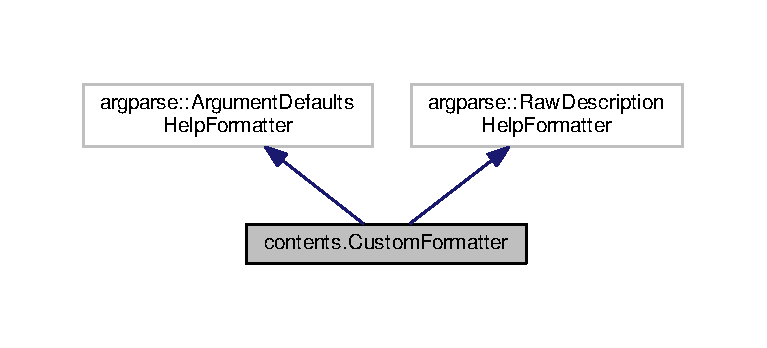
\includegraphics[width=350pt]{classcontents_1_1CustomFormatter__inherit__graph}
\end{center}
\end{figure}


Collaboration diagram for contents.\+Custom\+Formatter\+:
\nopagebreak
\begin{figure}[H]
\begin{center}
\leavevmode
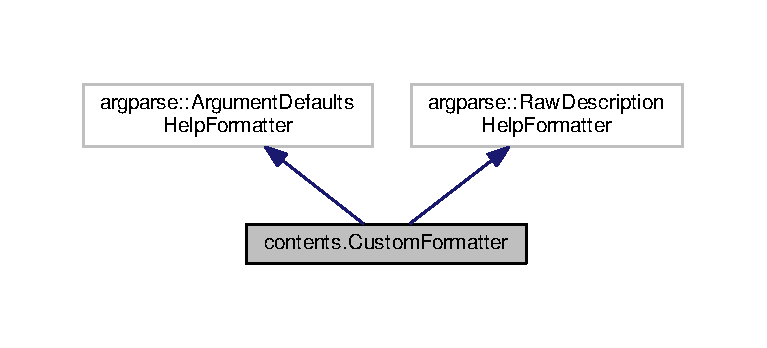
\includegraphics[width=350pt]{classcontents_1_1CustomFormatter__coll__graph}
\end{center}
\end{figure}


\subsection{Detailed Description}
Just a \hyperlink{classcontents_1_1CustomFormatter}{Custom\+Formatter}. 

Internally used only. \begin{DoxyVerb}Just a CustomFormatter.
\end{DoxyVerb}
 

The documentation for this class was generated from the following file\+:\begin{DoxyCompactItemize}
\item 
contents.\+py\end{DoxyCompactItemize}

%--- End generated contents ---

% Index
\newpage
\phantomsection
\addcontentsline{toc}{chapter}{Index}
\printindex

\end{document}
